\chapter{External specification}

\section{Hardware and software requirements}

Depending on whether one wants to use the user interface via a web browser or host the server themselves there are different requirements for each part.

\subsection{Browser}

The user interface requires a modern browser with JavaScript enabled. It is possible to use the system without JS, but theme switching and dropdowns in the navigation bar will not work.

On desktop the latest stable versions of the following browsers are supported:

\begin{itemize}
    \item Google Chrome
    \item Microsoft Edge
    \item Firefox and Firefox ESR
    \item Opera
    \item Safari (macOS only)
\end{itemize}

On Android and iOS support is restricted to the latest stable versions of:

\begin{itemize}
    \item Google Chrome
    \item Firefox
    \item Safari (iOS only)
    \item Android Browser and WebView (Android only)
\end{itemize}

Different and older browsers may work, but compatibility is not guaranteed.

\subsection{Server software} \label{chap:server-soft}

The server software requires the following external software to be installed:

\begin{itemize}
    \item Node.js 18.x or newer (not as a \href{https://snapcraft.io/node}{snap})
    \item MongoDB 6.0
    \item Docker Engine 20.10
    \item nginx 1.23.2 or newer
\end{itemize}

Supported operating systems:

% https://github.com/ranisalt/node-argon2/tree/v0.30.3#prebuilt-binaries
\begin{itemize}
    \item Ubuntu 20.04 or newer (x86-64, arm64)
    \item macOS 11 (x86-64), 12 or newer (x86-64, arm64)
    \item Windows 10 1809 or newer (x86-64)
    \item Windows Server 2019 or newer (x86-64)
\end{itemize}

It may be possible to run the server on other operating systems and architectures as long as the required software can be installed. These unsupported systems, however, will probably require \href{https://github.com/ranisalt/node-argon2/tree/v0.30.3#before-installing}{additional installation steps} related to \texttt{argon2} package setup.

\textbf{Warning:} Challenge Docker images must be compatible with the server architecture. Images presented in this project support only x86-64.

\section{Server installation}

The process of server software installation and configuration can be summarised in the following steps:

\begin{enumerate}
    \item Install the required software as described in section \ref{chap:server-soft}.
    \item Obtain the code from GitHub:\\
    \mintinline{bash}|git clone https://github.com/krzysdz/inz.git|
    \item Navigate to the downloaded project directory:\\
    \mintinline{bash}|cd inz|
    \item Install required npm packages:\\
    \mintinline{bash}|npm install --omit=dev|
    \item Configure MongoDB as a replica set (\href{https://www.mongodb.com/docs/manual/tutorial/deploy-replica-set/}{tutorial}).
    \item Configure the DNS to point the main domain and the challenges domain to the server. Example DNS configuration:
    \begin{mintedlexer}{DNSLexer.py:DNSLexer}
main-ui.com.        60  IN A        127.0.0.1
*.challenges.com.   60  IN CNAME    main-ui.com.
    \end{mintedlexer}
    \item Obtain TLS certificate for the main domain and the challenges domain. One certificate should cover both domains (the second one with wildcard).\\
    The key and certificate files should be placed in \texttt{nginx/certs} and named according to instructions from the \texttt{README} file in that directory.
    \item Adjust values in the \texttt{config.js} file.
    \item Start nginx with prefix set to \texttt{./nginx} and configuration \texttt{nginx/conf/nginx.conf}:\\
    \mintinline{bash}|nginx -p ./nginx -c ./nginx/conf/nginx.conf|
    \item Set \texttt{NODE\_ENV} to production:

    Bash/dash/zsh/csh:\\
    \mintinline{bash}|export NODE_ENV="production"|

    Powershell:\\%TC:ignore
    \mintinline{pwsh}|$env:NODE_ENV="production"|%TC:endignore
    \item Start the server:\\
    \mintinline{bash}|node index.js|

    \item \textit{Optional.} Configure services to automatically start the software. Example configuration for systemd based operating systems:
    \begin{enumerate}
        \item Modify the default mongod.conf file to specify replica set name as shown on Fig. \ref{fig:example-mongod} and enable the \href{https://github.com/mongodb/mongo/blob/e4fff3e1fe7b31b25cedde7b05205325b47b4a7d/debian/mongod.service}{mongod service}:\\
        \mintinline{bash}|systemctl enable mongod|
        \item Create a unit file for the proxy. An example is presented on Fig. \ref{fig:example-nginx-service}.
        \item Create a unit file for the main server. An example is presented on Fig. \ref{fig:example-server-service}.
        \item Enable and start the services:
        \begin{minted}{bash}
# Reload systemd configuration to pick up the new services
systemctl daemon-reload
# Enable the services to run at boot
systemctl enable inz-nginx
systemctl enable inz
# Start the server and proxy (required by inz.service)
systemctl start inz
        \end{minted}
    \end{enumerate}
\end{enumerate}

\section{Initial configuration}

If setting up the server with a fresh database, an administrator account must be created. To do this, one has to:

\begin{itemize}
    \item Create a user account (\texttt{/auth/register}).
    \item Set the \texttt{role} field of the user document to string \texttt{admin}. A Node.js script which does that is presented on Fig. \ref{fig:make-admin-script}.
    \item Log in into the account again.
\end{itemize}

\section{Types of users}
\label{chap:types-of-users}

There are three types of users considered in the system:

\begin{itemize}
    \item anonymous/not signed in
    \item regular users - account with role \texttt{"user"}
    \item administrators - account with role \texttt{"admin"}
\end{itemize}

Anonymous users can freely browse the application, but have a limited functionality on the task page.\\
Regular users gain access to profile page and unlock challenge and quiz submissions.\\
Administrators expand on the regular user permissions and can use an administration panel for managing the system.

\section{User manual}

This manual is intended for the end users. The functionality available for administrators is described in section \ref{chap:system-administration}.

\subsection{Theme selection}

The system can use light or dark mode acording to user preferences. By default the browser or OS determines the theme. A dropdown (Fig. \ref{fig:manual-theme}) shown after clicking an icon in the upper right corner can be used to manually change the page theme. The preference is stored in the browser. Three options are available:

\begin{itemize}
    \item Light - shown on Fig. \ref{fig:manual-theme-light},
    \item Dark - visible on Fig. \ref{fig:manual-theme-auto},
    \item Auto - determined by browser or OS preferences, presented on Fig. \ref{fig:manual-theme-auto} with browser theme set to dark.
\end{itemize}

\begin{figure}
    \centering
    \begin{subfigure}{0.48\textwidth}
        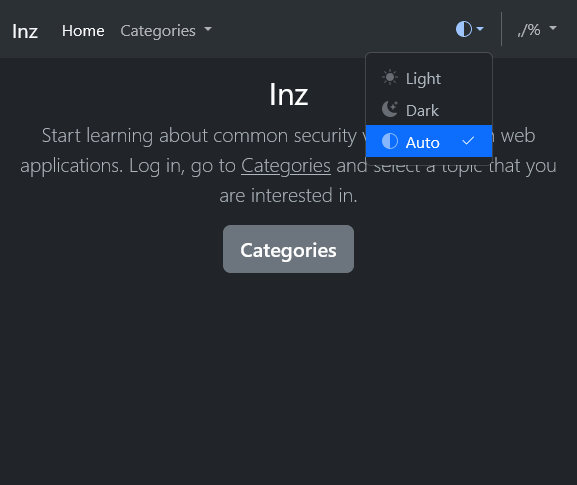
\includegraphics[width=\textwidth]{img/manual-theme-auto.png}
        \caption{Automatic theme - dark}
        \label{fig:manual-theme-auto}
    \end{subfigure}
    \hfill
    \begin{subfigure}{0.48\textwidth}
        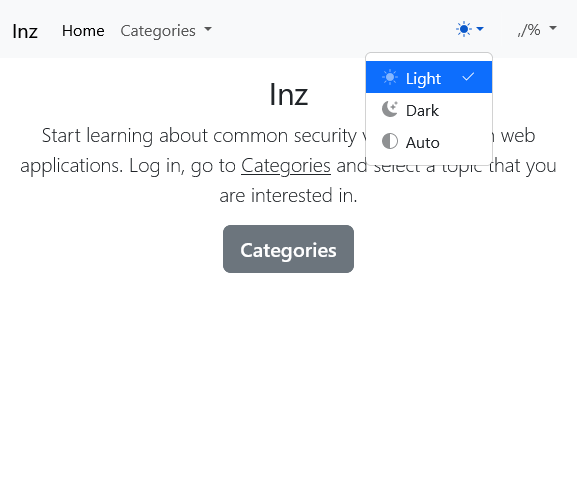
\includegraphics[width=\textwidth]{img/manual-theme-light.png}
        \caption{Light theme}
        \label{fig:manual-theme-light}
    \end{subfigure}
    \caption{Theme selection dropdown}
    \label{fig:manual-theme}
\end{figure}

\subsection{Account creation}
\label{chap:account-creation}

To access all features of the system a user account is required. Without it flag submission and later stages of solving tasks are impossible.

The account can be created on the \textit{Register} page which can be accessed from the home page as shown on Fig. \ref{fig:manual-home} or by clicking \textit{Create an account} on the login page. On that page the desired username and password have to be filled into the input fields. The password has to be between 8 and 64 characters long. To prevent mistakes in the password it has to be entered twice. If the passwords do not match the browser will prevent form submission and display an appropriate error.

The registration may fail if there already exists an account with the provided username. In such case a different username should be used.

\begin{figure}
    \centering
    \begin{minipage}{0.48\textwidth}
        \centering
        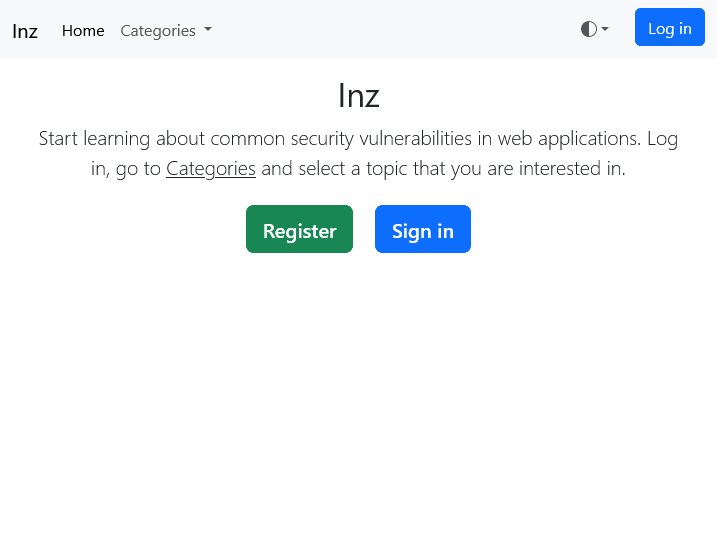
\includegraphics[width=\textwidth]{img/manual-home.png}
        \caption{Home page - logged out.}
        \label{fig:manual-home}
    \end{minipage}
    \hfill
    \begin{minipage}{0.48\textwidth}
        \centering
        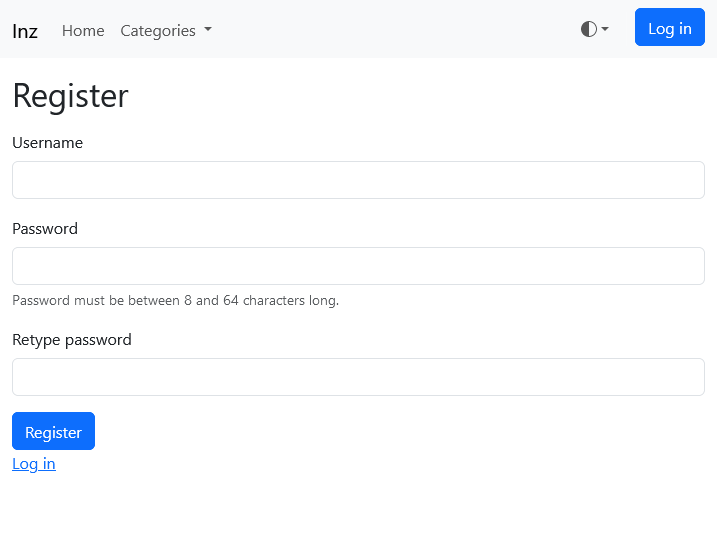
\includegraphics[width=\textwidth]{img/manual-registration.png}
        \caption{The registration page.}
        \label{fig:manual-registration}
    \end{minipage}
\end{figure}

\subsection{Logging in}

To use the account created in \ref{chap:account-creation} one has to log in into the account. To do that the user has to submit their username and password using a form on the login page (shown on Fig. \ref{fig:manual-login}). The page can be accessed by clicking a button in the navbar, a button on the home page or a link on the registration page.

\begin{figure}
    \centering
    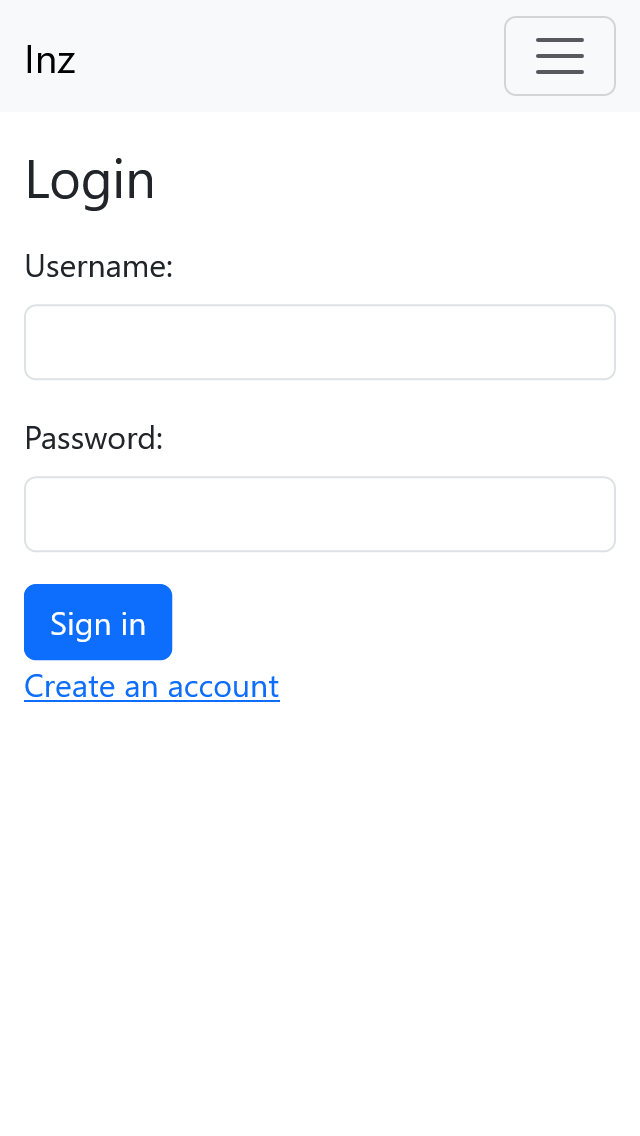
\includegraphics[width=0.4\textwidth]{img/manual-login.png}
    \caption{Login page viewed on mobile}
    \label{fig:manual-login}
\end{figure}

\subsection{Logging out}

A logged in user can log out using the \textit{Log out} button in the dorpdown appearing after the username in upper right corner is clicked. The dropdown is presented on Fig. \ref{fig:manual-home-dropdown-user}.

\begin{figure}
    \centering
    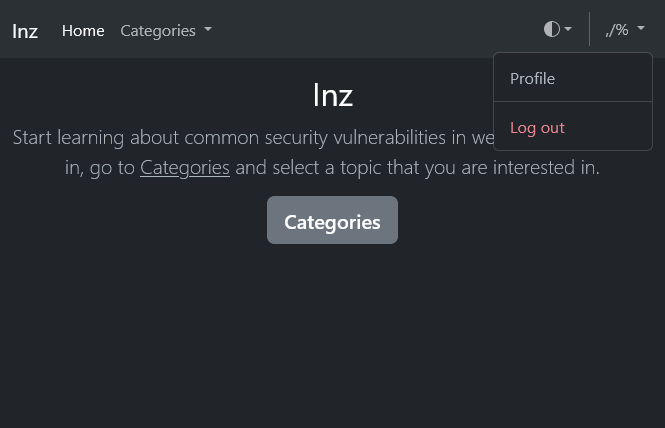
\includegraphics[width=\textwidth]{img/manual-home-dropdown-user.png}
    \caption{Username dropdown on home page for a regular user.}
    \label{fig:manual-home-dropdown-user}
\end{figure}

\subsection{Account management}

The profile page (\texttt{/profile}) shown on Fig. \ref{fig:manual-profile} is available for logged-in users through a link in the navbar (see Fig. \ref{fig:manual-home-dropdown-user}). This page allows changing the account password. To change the password one has to provide their current password and enter the new one two times. After submitting the form the system will show a message informing about the success or failure of the operation. Password change does not invalidate existing sessions.

\begin{figure}
    \centering
    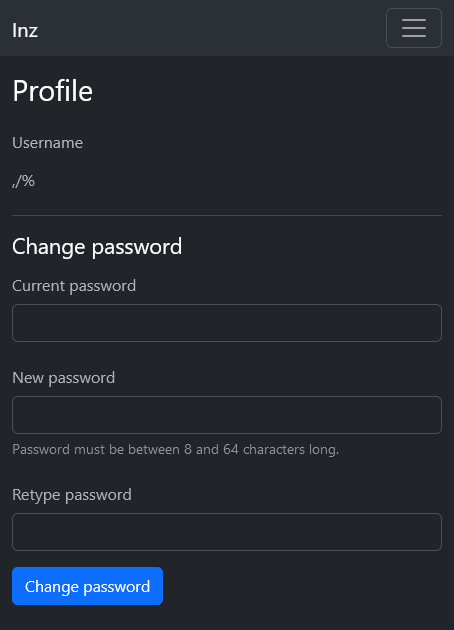
\includegraphics{img/manual-profile.png}
    \caption{Profile page in a narrow window.}
    \label{fig:manual-profile}
\end{figure}

\subsection{Browsing categories}

Categories in the system describe classes of vulnerabilities. A list of available categories can be accessed from the \textit{Categories} dropdown in navbar and from the \textit{Categories} (\texttt{/categories}) page. Both lists contain names of the categories which link to appropriate category pages.

% TODO: Insert dropdown and categories list page screenshots

Category pages describe classes of vulnerabilities, why these exist and how they can be avoided. Additionally, on the bottom of each category page there is a list of related tasks which demonstrate examples of such issues.

\subsection{Tasks}

Tasks show specific examples of vulnerabilities. Each task contains a link to a challenge website which has to be exploited. The process will look differently for each challenge. As a result of a successful attack the user should obtain a flag. The flags should follow the \texttt{flag\{xxx\}} scheme unless specified otherwise in the task description. Tasks can contain hints which may help in case of problems when solving the linked challenge. The hints are collapsed by default to avoid spoilers and can be uncovered by clicking them.

Once the flag is found it should be submitted on the task page. The form is shown only if the challenge is not solved. After a successful submission a message and a question appear instead of the form.

The second step of completing a task is answering a question. Questions are related to the challenge and usually concern avoiding the problem or fixing it. There are multiple answers, each of which can be marked as true by marking the checkbox next to it. Conversely, if an answer is thought to be false the checkbox should be left empty. Finally, the answers should be sent by clicking the \textit{Submit} button.

If the question has been answered the checkboxes are disabled and reflect user's choices. Answers correctly marked as true or false are displayed in green, while incorrect are shown in red. Additionally, the true answers are listed on the bottom of the page. Below some answers an explanation may appear which expands on the answer.

Selected incorrect answers may contain additional challenges. Below these answers a link to the challenge will appear. These challenges are modified versions of the original challenge. After solving such challenge the obtained flag should be submitted using a form below the answer.

\section{System administration}
\label{chap:system-administration}

The system is managed using and administrator panel \texttt{/admin}. It can be accessed from the dropdown in upper-right corner. JavaScript is strictly required for all functionalities of the panel. There are three tabs for different categories of administrative capabilities.

\subsection{Managing users}

The \textit{Users} tab offers basic account management features. In this tab a list of users registered in the system is presented. Next to each username their role is displayed. Finally, in the third column there are two action buttons. The first one changes user role from \texttt{user} to \texttt{admin} or the other way. The second one can be used to delete a user account. The list contains at most 10 entries. Pagination buttons below the table can be used to display another page of users.

\subsection{Managing categories}
\label{ssec:managing-categories}

The next tab \textit{Categories} allows creating and editing category pages. All existing categories are displayed as collapsed accordion items. Clicking on them opens a preview of the category description with an \textit{Edit category} button.

New categories can be created by clicking the \textit{New category} button at the top of the tab. The button opens a simple editor which can be used to create new categories. The name and description must be filled before creating the category using the \textit{Create} button. The name must use plain text, since it will always be escaped before displaying. The description should be entered using Markdown. To help with writing in Markdown a preview mode can be toggled by clicking the \textit{Preview} button on the right above the description input.

If the \textit{Edit category} button at the bottom of category description the editor will be populated with the stored details. The editor is the same as the one for new categories, but instead of the \textit{Create} button, a \textit{Save} button will appear.

Both creating a new category as well as editing an existing one causes reloading of the categories list. The description editor uses Marked for compiling Markdown content. The supported specification is listed at the bottom the discussion \href{https://github.com/markedjs/marked/discussions/1202}{markedjs/marked\#1202}.

\subsection{Managing tasks}
\label{ssec:managing-tasks}

The tab \textit{Tasks} show an overview of existing tasks and allows creating new. Like categories the existing tasks are listed as expandable accordion items.

New tasks can be added using a form which appears after clicking the \textit{New task} button at the to of the tab. The following data should be entered in the form:

\begin{itemize}
    \item \textbf{Task name:} The task name. It is displayed on the top of the task page and as a tile title on the bottom of relevant category page.
    \item \textbf{Category:} The category of vulnerabilities this task is assigned to. Must be chosen from one of the existing categories.
    \item \textbf{Description:} Task description displayed on the task page. The editor supports markdown and can be used the same way as the category description editor.
    \item \textbf{Challenge details:} The details for the main challenge. These options include:
    \begin{itemize}
        \item \textbf{Docker image:} Docker image to use for the challenge container. The image will be pulled after creating the task.
        \item \textbf{Subdomain:} Subdomain of the domain specified in the config file, which will be used to hosting the challenge.
        \item \textbf{Flag:} Flag which should be found by the users. Flags submitted by users will be compared to this value.
        \item \textbf{Expose flag as \texttt{FLAG} environmental variable:} Whether the flag should be exposed in the container as an environmental variable \texttt{FLAG}. This option can be used to avoid hardcoding flag values in challenge images.
        \item \textbf{Reset interval:} How often the challenge container should be removed and recreated. The value should be given in seconds. Set to 0 to disable automated restarts.
    \end{itemize}
    \item \textbf{Hints:} A list of hints for the main challenge. Hints are rendered inside a collapsed \mintinline{html}|<details>| tag on the task page, because they are supposed to contain \textit{spoilers}. New hints can be added by clicking \textit{Add a hint}. All hint inputs must be filled. The X button on the right of a hint input can be used to remove it. It is possible to create a task with no hints.
    \item \textbf{Question:} The question shown after solving the challenge. The question is rendered without escaping, so inline HTML can be used, but the content is placed inside an \mintinline{html}|<h4>| tag.
    \item \textbf{Answers:} These are the answers to the question from the field above. Additional answers can be added using the \textit{Add an answer} button. It is not possible to remove an answer. An answer has the following properties:
    \begin{itemize}
        \item \textbf{Answer:} The answer text that is presented to the users. The text is not escaped and can include HTML.
        \item \textbf{Answer is correct:} Whether the answer is correct and users are expected to check it.
        \item \textbf{Add challenge:} Shows an additional set of fields related to an extra challenge. \textbf{Available only if the answer is not marked as correct.}
        \item \textbf{Explanation:} An \textbf{optional} explanation that is shown after answering the question. It may underline the reasons why an answer is right or wrong.
        \item \textbf{Challenge details:} Challenge details for an additional challenge related to the answer. Options are the same as for the main challenge. \textbf{Shown only if the \textit{Add challenge} option is checked.}
    \end{itemize}
\end{itemize}

An expanded task accordion item presents the task properties. Challenge details other than the \textit{expose flag...} option are shown in collapsed \mintinline{html}|<details>|. Checkboxes next to answers indicate whether these answers are marked as correct. Optional explanations are shown in italics below respective answers.

\section{Security issues}

Secure design is an important part of the project. The target audience is expected to be or become experienced with exploitation, so the system had to be carefully created and must be responsibly managed.

\subsection{Project author's considerations}

Security of the system in a huge part depends on the main server design and implementation details.

\subsubsection{Data flow analysis}

The data sources provided by regular users are:

\begin{itemize}
    \item username set in the registration process - a string of at most 255 characters, always escaped in templates, inserted as \texttt{textContent} in admin panel, encoded with \mintinline{js}|encodeURIComponent()| in URLs,
    \item category name - a string (part of the URL), used for comparison in \texttt{\$match} stage of an aggregation pipeline as %TC:ignore
    \mintinline{js}|{ $match: { name: name } }|%TC:endignore
    ,
    \item task id and challenge id in challenge and quiz submissions - always a conversion to \texttt{ObjectId} is attempted, only the converted value is used later,
    \item flag in challenge solution submission - trimmed using \mintinline{js}|String.prototype.trim()| and compared using \mintinline{js}|===|,
    \item \texttt{answer[n]} properties in quiz submission - iterated from 0 to the number of answers in the task and compared to \mintinline{js}|"on"|.
\end{itemize}

The data coming from these sources is always used in a safe way. Data entered by administrators can be \textit{dangerous} by design, since they must be able to insert raw HTML and run any software using containers.

\subsubsection{Known vulnerabilities}

Express version used in the project depends on a vulnerable version of qs library (\href{https://www.cve.org/CVERecord?id=CVE-2022-24999}{CVE-2022-24999}). qs package is used in Express only if the \texttt{query parser} setting is set to \mintinline{js}|"extended"| or the \texttt{urlencoded} middleware's \texttt{extended} option is a truthy value. The \texttt{query parser} option is \mintinline{js}|"simple"| by default and the \texttt{urlencoded} middleware is created with \mintinline{js}|{ extended: false }|, so this vulnerability should not affect the project.

\subsection{Administrator's responsibilities}

Regardless of the project design it has to be configured and used properly so as not to introduce new security issues. System administrators should keep in mind the following warnings:

\begin{itemize}
    \item  Challenges should use a different domain than the main website so that users who exploit a challenge will not be able to set cookies valid for the main domain.
    \item Special care must be taken when designing challenges, especially ones leading to RCE. Since challenges are running as Docker containers a misbehaving container can bring the whole system down. To provide isolation and limit resources use of \href{https://github.com/google/nsjail}{nsjail} is suggested.
\end{itemize}

\section{Covered categories of issues}

The design of the project separates the system from the content. Categories and tasks can be added at any time as described in sections \ref{ssec:managing-categories} and \ref{ssec:managing-tasks}. The example deployment covers some of common security vulnerabilities found in web applications.

\subsection{SQL injection}

This category covers basics of SQL injection exploitation and prevention. Small code snippets and examples are provided to help users understand the reason behind this class of vulnerabilities. At the bottom of the description a \textit{Read more} section contains links to additional resources connected to this topic.

An example of a vulnerable application is presented in the \textit{Private todo} task. The target is a simple website offering TODO list creation and sharing. These lists are accessed using an \texttt{id} parameter, which is insecurely concatenated with the database query allowing for an injection attack. The question shown after solving the challenge presents the vulnerable line and answers show suggested methods of fixing the problem. One of them which proposes filtering some SQL keywords has an additional challenge.
